% June 2015 (TOC contents linked in blue in pdf file)
%This template was prepared by Dorothea F. Brosius of the 
%Institute for Electronics and Applied Physics, University of Maryland, College Park, MD
%The template was last updated in June 2015
%Thesis Main Page used with thesis.sty based on the
%University of Maryland Electronic Thesis and Dissertation (ETD) Style Guide (2014)

%The YourInformation file was created by Freja Nordsiek, 2014.
%Code for linking the TOC titles to the text in the pdf file was created by Freja Nordsiek, 2014.


% Select the version that fits how you are making this LaTeX document (its driver).
% The first two are the most likely ones to be needed.
%
\newcommand{\mydriver}{pdftex} %Making a PDF directly using pdflatex.
%\newcommand{\mydriver}{dvipdfmx} %Making a DVI and converting that to PDF using dvipdfmx.
% \newcommand{\mydriver}{dvipdfm} %Making a DVI and converting that to PDF using dvipdfm.
% \newcommand{\mydriver}{dvips} %Making a DVI and converting that to PS using dvips (may later be converted to PDF).  (Used with my pc)
% \newcommand{\mydriver}{dvipsone} %Making a DVI and converting that to PS using dvipsone (may later be converted to PDF).
% \newcommand{\mydriver}{ps2pdf} %Same as the one for dvips except it is compatible with Ghostscript's PDF writer.


\documentclass[12pt,\mydriver]{thesis}  %12pt is larger than 11pt

\usepackage{titlesec}
   \titleformat{\chapter}
      {\normalfont\large}{Chapter \thechapter:}{1em}{}

\usepackage{graphicx}
\usepackage{epstopdf}
\epstopdfsetup{update} % only regenerate pdf files when eps file is newer
\usepackage{cite}
\usepackage{lscape}
\usepackage{indentfirst}
\usepackage{latexsym}
%\usepackage{amsmath}
\usepackage{multirow}
\usepackage{tabls}
\usepackage{wrapfig}
\usepackage{slashbox}
\usepackage{longtable}
\usepackage{supertabular}
%\usepackage{subfig} % make it possible to include more than one captioned figure/table in a single float
\usepackage{subeqn}
\usepackage{subfigure}
\usepackage[pdftex, bookmarks, colorlinks=true, plainpages=false, citecolor=blue, urlcolor=blue, filecolor=blue, linkcolor=blue]{hyperref} 
	%Works with PcTex.  You may have to choose one of the drivers above if dvips does not work.

\newcommand{\tbsp}{\rule{0pt}{18pt}} %used to get a vertical distance after \hline
\renewcommand{\baselinestretch}{2}
\setlength{\textwidth}{5.9in}
\setlength{\textheight}{9in}
\setlength{\topmargin}{-.50in}
%\setlength{\topmargin}{0in}    %use this setting if the printer makes the the top margin 1/2 inch instead of 1 inch
\setlength{\oddsidemargin}{.55in}
\setlength{\parindent}{.4in}


\begin{document}

\pagestyle{plain}
\pagenumbering{roman}
\setcounter{page}{2}

\setlength{\parskip}{0em}
\renewcommand{\baselinestretch}{2}
\small\normalsize

%Pages from this point start at Arabic numeral 1
\setcounter{page}{1}
\pagenumbering{arabic}
%Chapter 3

\renewcommand{\thechapter}{3}

\chapter{Centroid Steering}

\section{Motivation}



\section{Considerations for low-ridgidity electron beam}


\begin{figure}
\begin{center}
\includegraphics[width=\textwidth]{3.figures/Earth_field.png}
\end{center}
\renewcommand{\baselinestretch}{1}
\small\normalsize
\begin{quote}
\caption[Figure with caption indented]{Measured Earth field, from Dave Sutter measurements 6/1/2010. Red dashed = radial field (positive = outward direction). Blue solid = vertical field.}
\label{fig:earthfield}
\end{quote}
\end{figure} 
\renewcommand{\baselinestretch}{2}
\small\normalsize


\section{Prior Approach}


% New Approach
This note describes the quad-as-BPM measurement procedure and a new steering algorithm designed to horizontally center the beam in the quadrupoles. 
The quad-as-BPM measurement, described in Section \ref{sec:quad_as_BPM}, was developed by Kiersten and Irv and measures the position of the beam 
on the first turn using quad scan data. The horizontal steering algorithm, Section \ref{sec:horz_steer}, is a methodical, "front to back" approach 
that first minimizes the position of the beam in the quadrupoles on the first turn then minimizes orbit deviations in subsequent turns. This is 
proposed as a alternative to the response matrix steering algorithm \cite{KPRnote:2011}, and may be more useful for applications where orbit 
centering in the quadrupoles is essential.


\section{Quadrupole as BPM technique}

The quad as BPM method is a way to measure the beam orbit in the first turn. We calculate the beam position at the center of 
each quadrupole by measuring the change in beam position due to a perturbation in the quadrupole current. 
This is an essentially identical method to that described by Kamal Poor Rezaei in an earlier technical note \cite{KPRnote:2012}, 
with the main difference being the use of the VRUMER beam tracking code to calibrate position, rather than a transfer matrix calculation.  


%% ADD MORE

In the work described here, calibration of quadrupole response (measured directly at nearest downstream BPM) is accomplished using VRUMER. VRUMER, described in detail in Appendix [TBD], 
is a simple orbit integrator written in Matlab, originally developed by Irv Haber to model transverse beam centroid behavior and test UMER-specific steering algorithms.
The model used here includes the measured background earth field, applied as a continuously 
acting, lab-frame-position dependent force based on linear interpolation between measurement points at the 36 dipoles.
This model does not include centroid kicks as a result of magnet fringe fields or the steering effect of the offset YQ magnet, although 
the framework can support these refinements.



\subsection{Avoiding null points} \label{sec:QAB:nulls}

Generally, the quad as BPM measurement uses response data from the nearest downstream BPM. However, for certain quad-BPM pairs this may not be appropriate due to the BPM being located near a null point of the betatron oscillation. 

There are two reasons why the BPM response will be very flat: the beam is near the center of the quadrupole, or quad-BPM separation is close to $n \frac{\lambda}{2}$ for integer n, where $\lambda$ is the betatron wavelength. The beam transformation in VRUMER is not exactly equivalent to the transformation in UMER (VRUMER does not include edge focusing, SC effects, etc). Therefore, quad-BPM separations near $n \frac{\lambda}{2}$, the BPM response slope will be small in both VRUMER and UMER but not identical. (This is true for all quad-BPM pairs, but will generally be a small error). 
%For a non-zero BPM response slope, the Newton Raphson calculation will tend to pick a very large $x_q$ for the simulation reponse to match the measured response. 

At an operating point of 1.826 A, the UMER 6 mA beam has $\nu_x = 6.636$, $\nu_y=6.752$ \cite{RKnote:2010}. This corresponds to betatron wavelengths $\lambda_x = 1.736$ m, $\lambda_y=1.706$ m.
In the VRUMER simulation, horizontal and vertical tunes are equal (no edge focusing), $\nu=6.293$, equivalently $\lambda = 1.83$ m. This is consistent with the simplifications made in VRUMER. 

We can see that the quad-BPM separations for which unusually high $x_q$, $y_q$ values appear (Table \ref{tab:nulls}) are close to the the VRUMER wavelength $\lambda = 1.83$ m, $\frac{\lambda}{2} = 0.92$ m. There are two inaccuracies that may result from this:

\begin{itemize}
\item Quad-BPM separation is close to UMER betatron wavelength (a null in the actual ring). VRUMER sees a small $\frac{\partial x_{BPM}}{\partial I_Q}$ slope and predicts $x_q \sim 0$, while in reality $x_q$ could be fairly large. This is hard to discern from the data, and may artifically obscure bad first-turn steering.
\item Quad-BPM separation is close to VRUMER betatron wavelength. If BPM response slope is not very flat (but VRUMER thinks this should be a null point) the VRUMER calculation for $x_q$ blows up. This can be seen in Fig. \ref{fig:nulls}, where QR14, QR32 and QR62 in particular have unphysically large $x_q$.  
\end{itemize}



\begin{table}
\centering
\caption{}
\label{tab:nulls}
\begin{tabular}{|c|c|c|c|c|}
Quad \# & Nearest BPM & $\Delta S_{Q \rightarrow BPM}$ [m] \\
\hline
QR14 & RC5 & 0.88   \\
QR32 & RC11 & 1.84 \\
QR38 & RC11 & 0.88 \\
QR62 & RC17 & 0.88  \\
QR70 & RC1 (turn 2) & 0.88  \\
\end{tabular}
\end{table}


% \begin{figure}
% \centering
% \caption{Quad as BPM data taken 6/9/15, position in each quad is determined by response in next downstream BPM. Solid circles are BPM data.}
% \label{fig:nulls}
% \includegraphics[width=\textwidth,trim={.7in 5.2in .7in 2.6in},clip]{figures/scan150609_withBPMdata_xy.pdf}
% \end{figure}

% \begin{figure}
% \centering
% \caption{Null point effect as seen in VRUMER simulation. Each trace represents a different simulation, where the strength of RQ14 is varied. The null point occurs near RC15 for both horizontal (top) and vertical (bottom). }
% \label{fig:nulls_vrumer}
% \includegraphics[width=\textwidth,trim={.7in 5.2in .7in 2.6in},clip]{figures/Q14_allBPMS_VRUMER_zoomin.pdf}
% \end{figure}


In subsequent quad as BPM data in this note, QR14, QR32 and QR62 use the BPM response in the next nearest downstream BPM to avoid artificial blow-up or suppression of $x_q$ and $y_q$. 
This effect should also be (but is not currently) included in the calculation of errorbars for the quad as BPM data.












\section{Ring steering}




\subsection{Horizontal Steering Procedure}

Using VRUMER, I explored the effectiveness of various minimization functions on the first-turn beam orbit for a variety of injection conditions and misalignments. The available minimization functions include steering through downstream focusing or defocusing quad (minimize position in a single quad) or minimization of an RMS quantity dependent on position in both downstream quads. In the thin lens approximation for a focusing dipole separated from a defocusing dipole by a drift of distance $L$, $x'_F = \frac{x_D-x_F}{L}$. I used $x'_F \propto x_D-x_F$ to include $x'_F$ in the RMS minimization term, see Table \ref{tab:algorithm}.

\begin{table}[h]
\centering
\caption{Different algorithms and their performance (RMS position in quads) for initial condition $x=1$mm, $x'=0$. }
\label{tab:algorithm}
\begin{tabular}{|l|l|c|c|c|}
\hline
shorthand & Minimization function & RMS($x_Q$) [mm] & RMS($x_Q$) [mm]  & plot trace \\
& & no misalign. & $\sigma=5$mm & \\
\hline
$x_F$ & $\| x_F \|$ & 5.3 & 37.3 & {\color{blue} $\circ$} \\
$x_D$ & $\| x_D \|$ & 0.2 & 6.9 & {\color{red} $\triangle$} \\
$x_F,\thinspace x_D$ & $\sqrt{x_F^2+x_D^2}$ &  2.1 & 9.3 & {\color{cyan} $\diamond$} \\
$x_F,\thinspace x'_F$ & $\sqrt{x_F^2+(x_D-x_F)^2}$ & 0.2 & 6.6 & $\ast$ \\
$x_D,\thinspace x'_F$ & $\sqrt{x_D^2+(x_D-x_F)^2}$  & 0.2 & 7.0 & {\color{magenta} $+$} \\
\hline
\end{tabular}
\end{table}




\begin{figure}[!htb]
\centering
\subfloat[No misalignments]{
	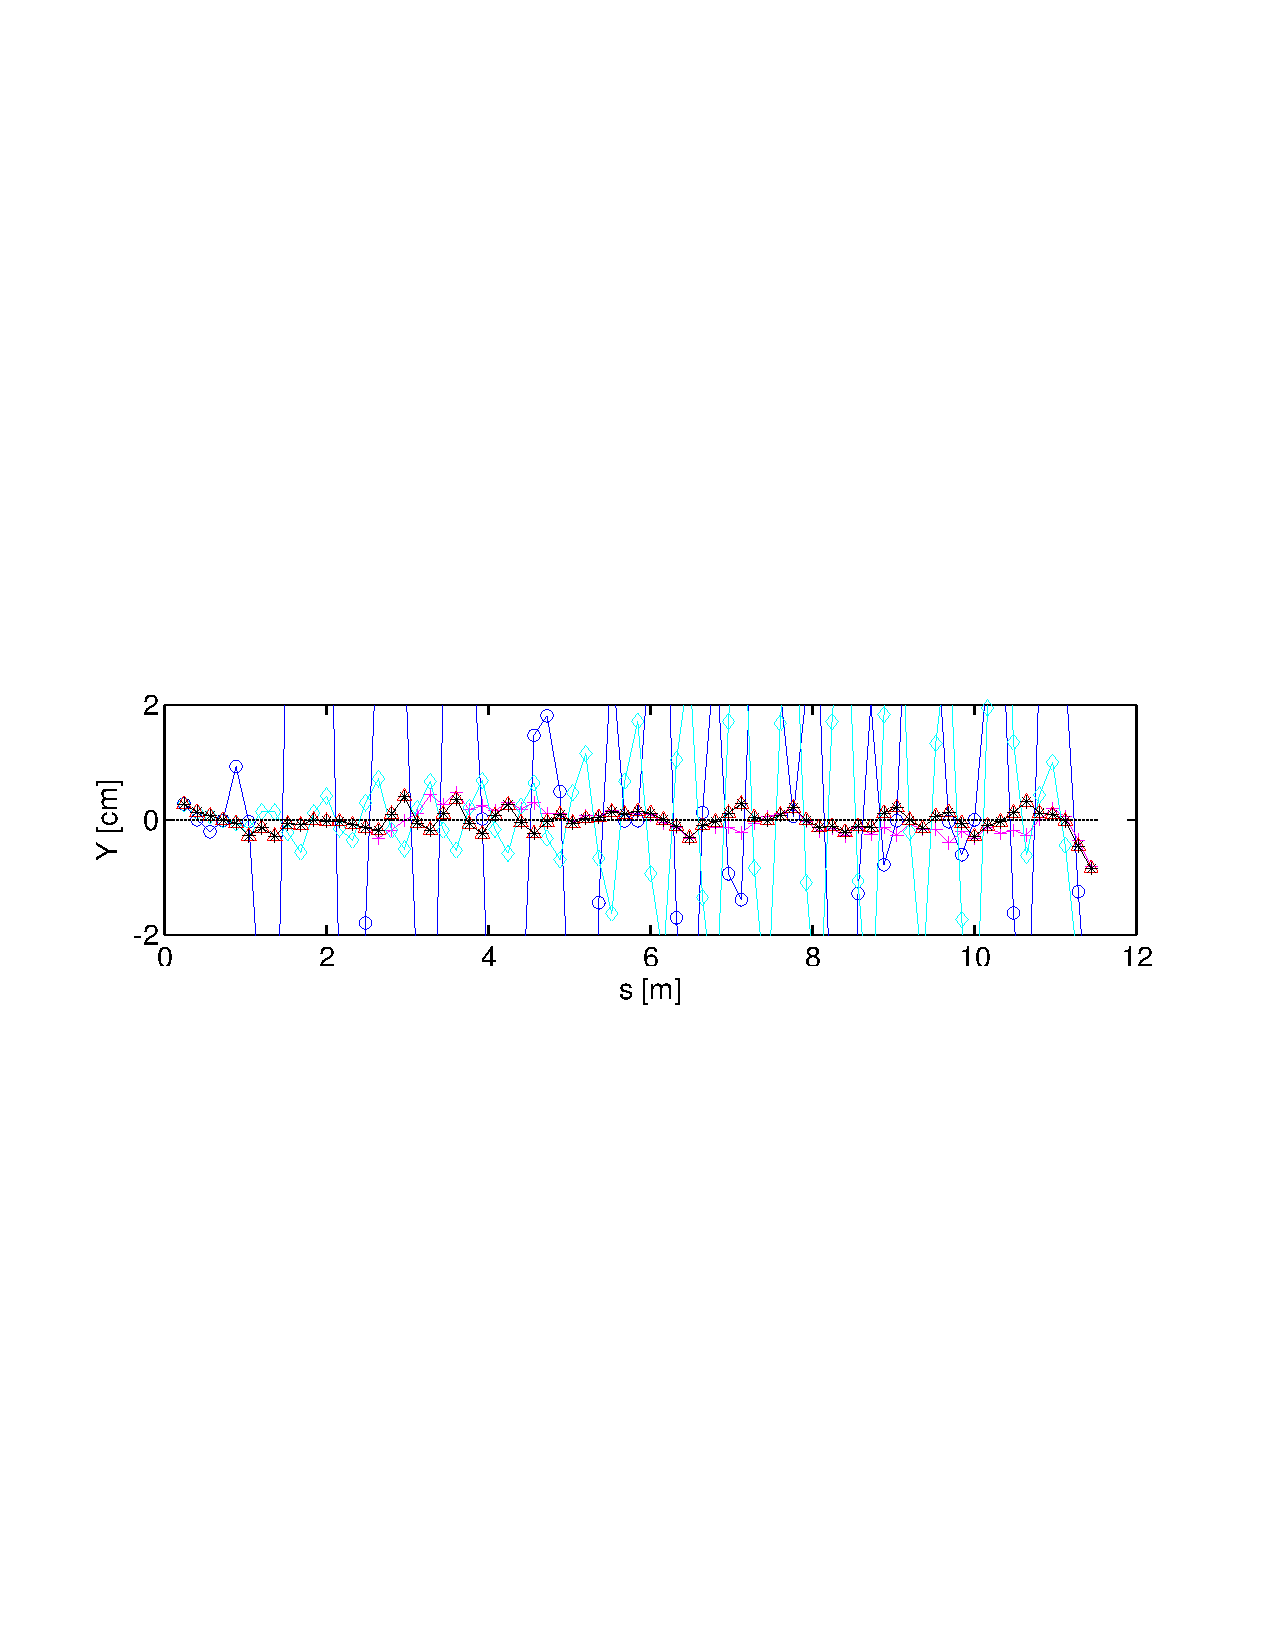
\includegraphics[width=\textwidth,trim={.5in 4.3in .7in 4.5in},clip]{3.figures/vrumer_steering_algorithm_compare_x1_xp0.pdf}}
\hspace{.05in}
\subfloat[Random quad misalignments from Gaussian distribution, $\sigma=5$mm]{
	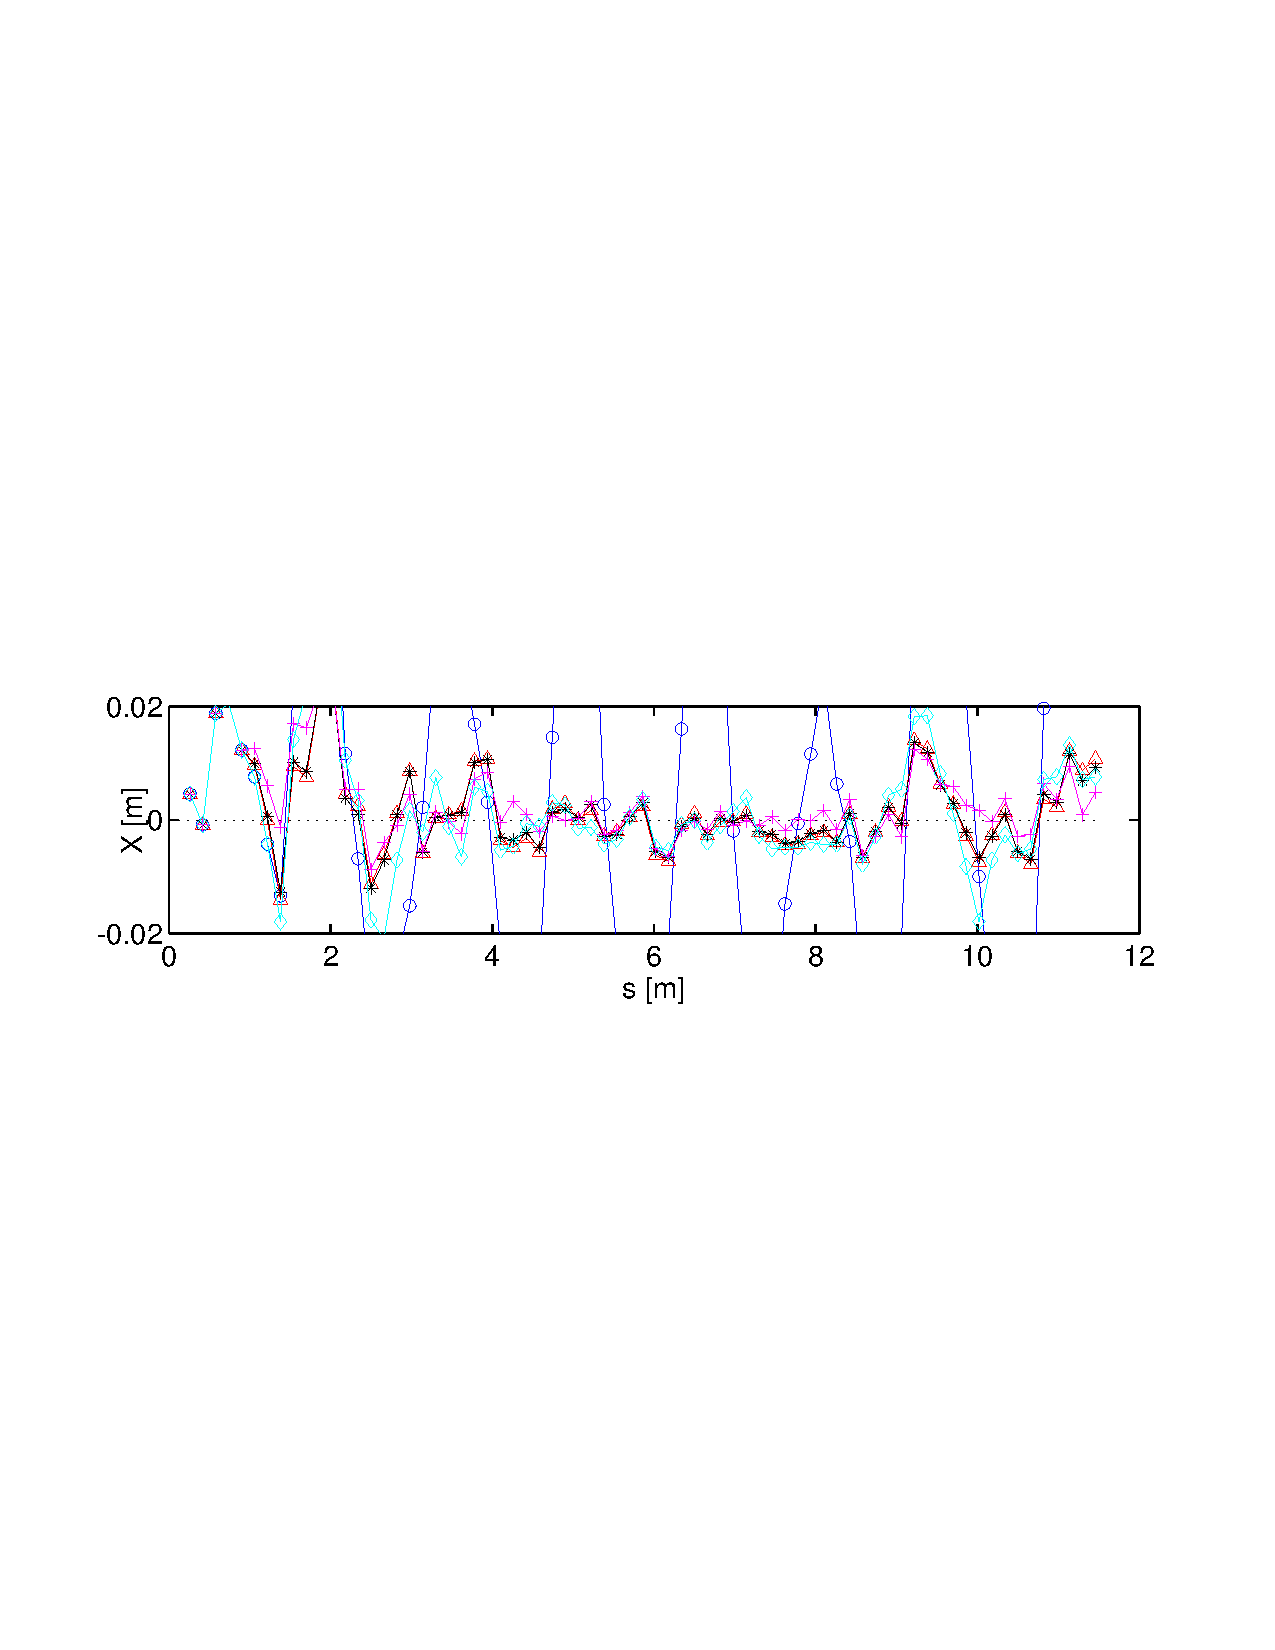
\includegraphics[width=\textwidth,trim={.5in 4.3in .7in 4.5in},clip]{3.figures/vrumer_steering_algorithm_compare_x1_xp0_sig5.pdf}}
\caption{First turn VRUMER orbits for initial condition $x=1$mm, $x'=0$. 
%blue circle: $x_F$, red triangle: $x_D$, black asterisk: $x_F$,$x'_F$, 
%magenta plus:  $x_F$,$x'_F$, green diamond: $x_F$,$x_D$
}
\label{fig:algorithm}
\end{figure}




Qualitatively, steering by $x_D$ and $x_F$,$x'_F$ result in almost identical orbits (sub-millimeter differences) that converge very quickly towards the center of the quads given an injection error or quad misalignment.
 In practice, it is much faster to minimize $x_D$, as that requires 1 quad scan for every dipole setting rather than 2 quad scans. It also allows interpolation between scanned dipole settings, as the data can be fit to a line and the zero-crossing calculated (the RMS minimization functions do not lend themselves to fitting by a simple function). However, the $x_F$,$x'_F$ algorithm seems to yield better results in the lab. 
This may be because of its ability to handle relative misalignments between the focusing and defocusing quadrupoles.

The caveats associated with using both of these algorithms will be further discussed in the following section.



\begin{figure}[!h]
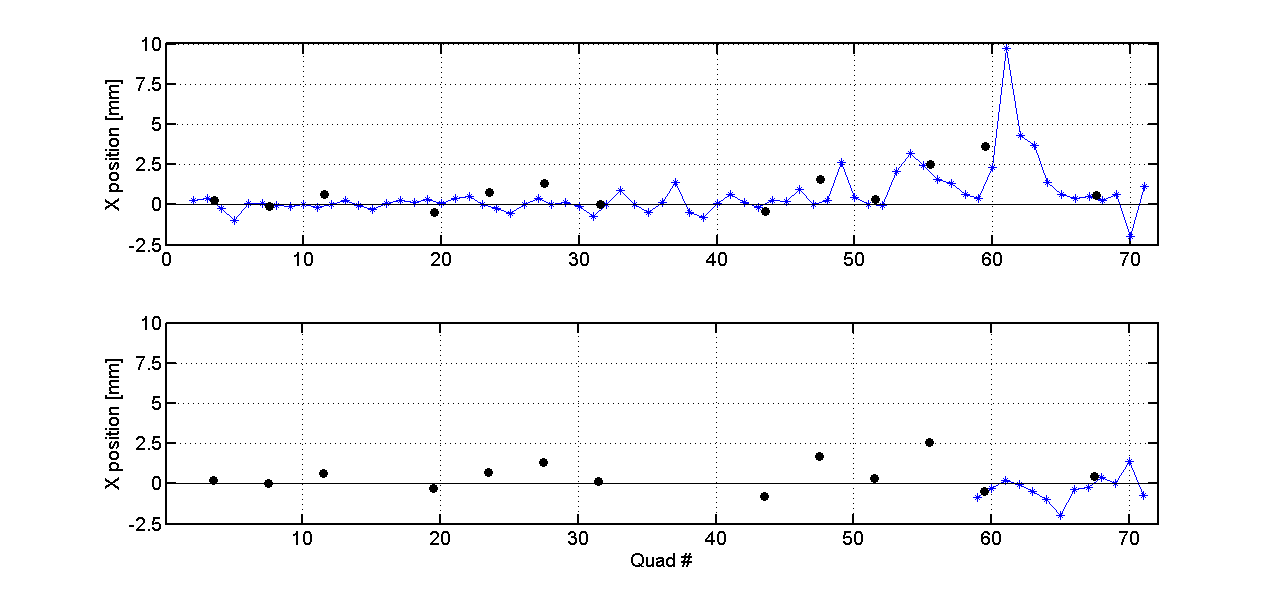
\includegraphics[width=\textwidth]{3.figures/quadscan_151113_151116.png}
\caption{1st turn solution generated on 11/13/15 (top) and 11/16/15 (bottom), by steering through defocusing quadrupoles.}
\label{fig:ring_steering}
\end{figure}


\begin{figure}[htb]
\centering
\subfloat[Position in defocusing quad]{\label{fig:ring_steering:xd}
	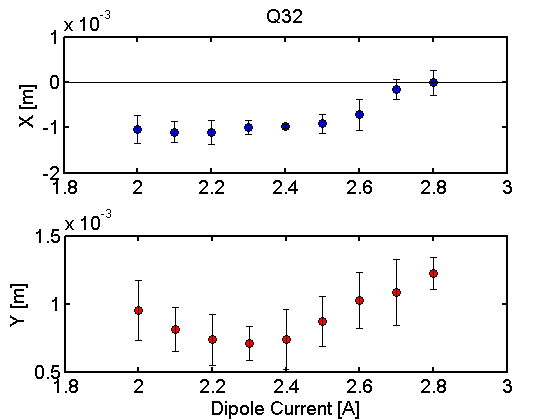
\includegraphics[width=0.45\textwidth]{3.figures/ring_steering_D15_it2_Q32.png}}
\hspace{.05in}
\subfloat[Position in focusing quad]{
	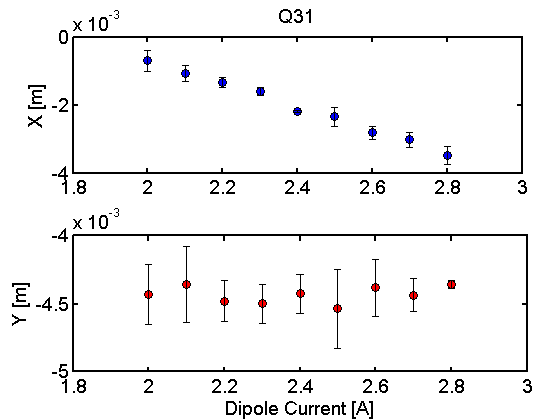
\includegraphics[width=0.45\textwidth]{3.figures/ring_steering_D15_it2_Q31.png}}
\hspace{.25in}
\raggedleft
\subfloat[RMS minimization of $x_F$ and $x_D-x_F$]{ \label{fig:ring_steering:rms}
	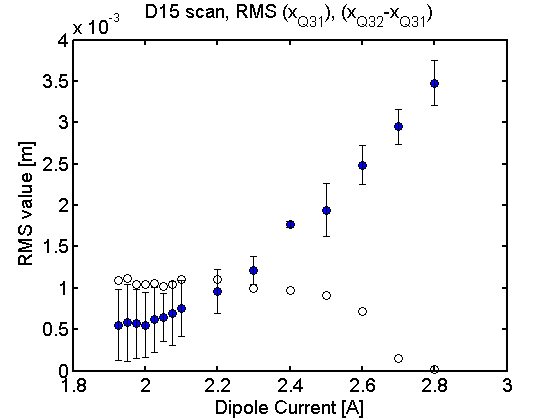
\includegraphics[width=0.45\textwidth]{3.figures/ring_steering_D15_RMS_it2.png}}

\caption{Steering through D15 using two different algorithms, 11/11/15}
\label{fig:injection_steering}
\end{figure}


%%% Point rejection algorithm
A weakness of the  $\| x_D \|$ minimization is that occasionally the data will not fall on a straight line. This is most likely due to scraping between the dipole and BPM or noise in the region near the pulser. In the ring steering scripts, I have implemented a points rejection critera that throws away quad position data with errorbar $> 1$ mm. As the quad position is proportional to the slope of the beam position in the BPM during the quad scan, the error bar is proportional to the uncertainty in the fitted slope -- large nonlinearities in the quad scan data will have large error bars bracketing the estimate of position in the quadrupole. However, some clearly nonlinear points do not have associated large error bars, and one can still get sidetracked by this effect.

The $x_F,\thinspace x'_F$ algorithm seems less likely to be led astray by nonlinear response in one of the quads. However, similar problems originating around D15 and D29 arose when using the $x_F$, $x'_F$ minimization, as seen in Fig. \ref{fig:QAB1}. This may be due to misalignments, but will likely be improved by stepping through the ring dipoles for a second steering iteration (at least from D15 onwards). 



\subsection{Vertical Steering Procedure}

\begin{figure}[h]
\centering
\subfloat[Vertical position of beam in quads for 1st turn.]{\label{fig:vertical_quads}
	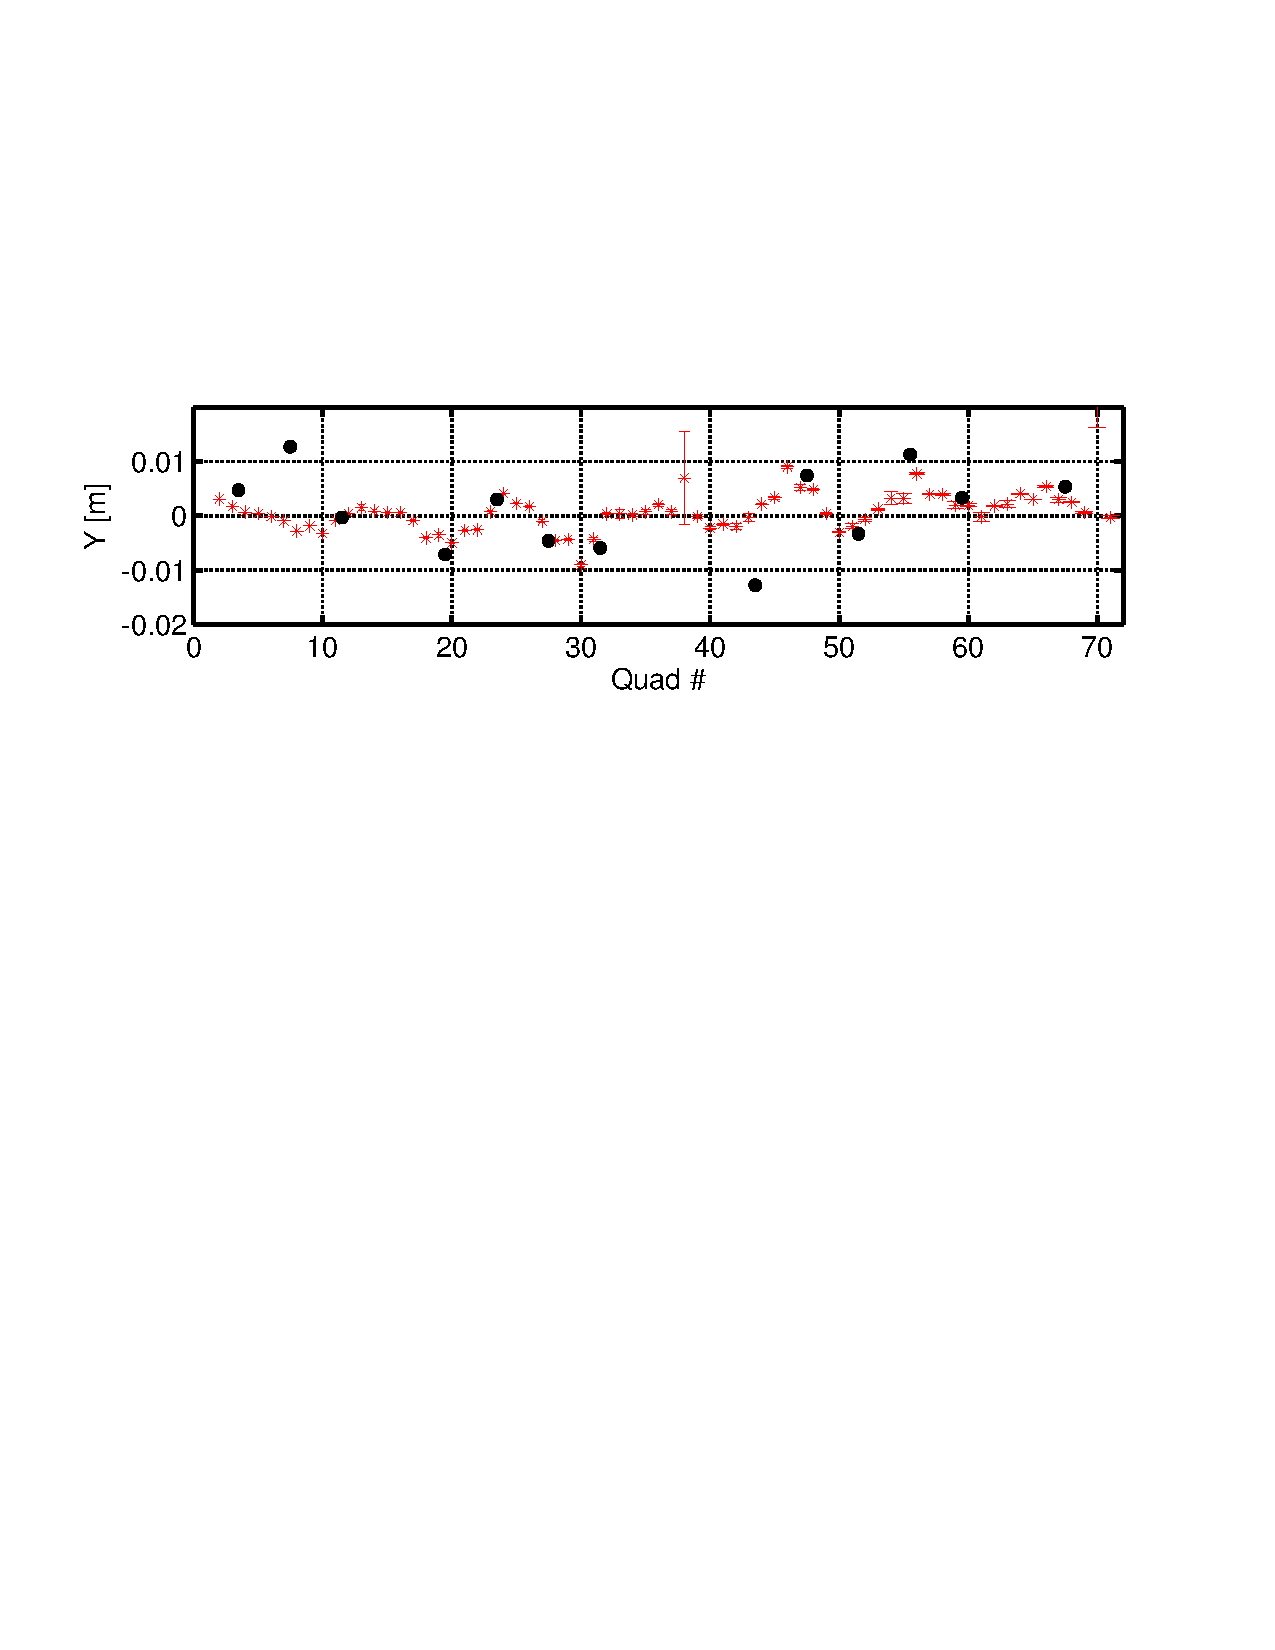
\includegraphics[width=\textwidth,trim={.5in 6.4in .5in 2.4in}, clip]{3.figures/quad_as_BPM_Y.pdf}}
\hspace{.05in}
\subfloat[Vertical position of beam in BPMs for first 4 turns. Note shorted vertical plates at RC2, RC11.]{\label{fig:vertical_BPMs}
	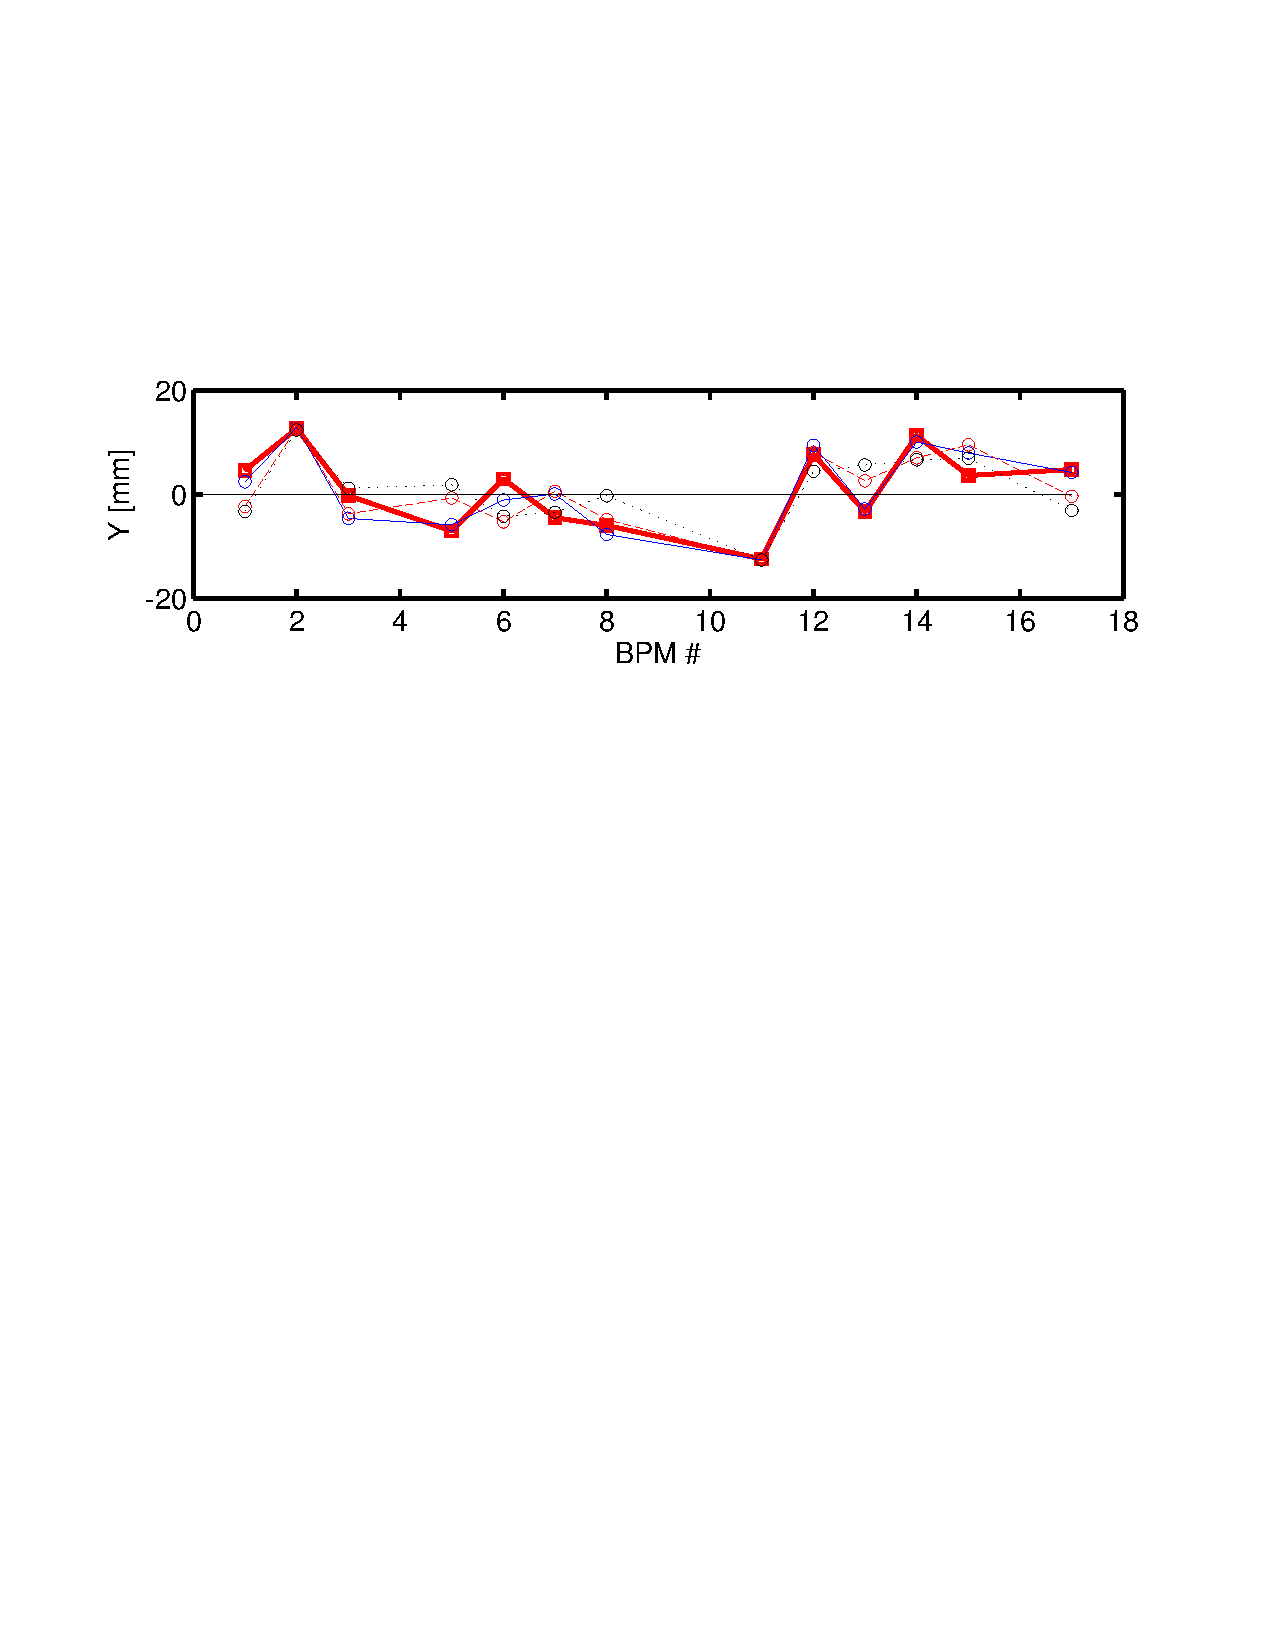
\includegraphics[width=\textwidth,trim={.5in 6.5in .5in 2.4in}, clip]{3.figures/BPM_position_sol151116_Y.pdf}}
\end{figure}

Vertical steering in UMER is accomplished by 18 vertical correction magnets located at the pipe flanges between plates. All of these magnets are fairly weak, due to the wide bore. With an integrated field of 3.886 G-cm/A, this gives a corrective kick with magntiude $0.66^{\circ}$/A. (For comparison, ring dipoles have a correction of $3.4^{\circ}$/A.) The largest source of vertical alignment errors is the radial component of the Earth's field, shown in Fig. \ref{fig:EarthField}. Although the amplitude 200 mGauss is comparable to the vertical field, the average is only $\sim3$ mGauss.

Previous assumption has been that sparsely populated, low-field vertical correctors were sufficient to correct for the low average radial field. Fig. \ref{fig:vertical_quads} and \ref{fig:vertical_BPMs} show measurement of typical vertical steering solution for the 6 mA beam. This solution was obtained by Brian using a trial and error method, settings are saved in kiersten\_6mA\_151116.csv. In the first turn, the maximum vertical displacement from quad center is 10 mm and the RMS displacement is 3.2 mm. Deviation about this orbit in the first 4 turns is $\sim10$ mm. 

This is much worse than the best horizontal steering solution described in this note. For horizontal beam position, the first-turn orbit (Fig. \ref{fig:ring_steering}) exhibited maximum horizontal displacement of 3.1 mm and RMS displacement of 0.8 mm. Deviation about this orbit in the first 4 turns is $\sim2$ mm. 


While good recirculation is possible using the existing correctors, an attempt to steer through the vertical center of the quads will inherently be limited by the strength and density of vertical correctors. We use VRUMER to test various vertical steering algorithms and place a lower bound on the best possible first turn orbit using existing vertical steerers, results are shown in Table \ref{tab:vert_algorithm}. This note considers three cases: 

\begin{itemize} 
\item Ideal: Perfect alignment, SV current constrained to be $\le10$ A. 
\item SV limit: Perfect alignment, SV current limited to $\le2$ A.
\item Misaligned: Random misalignment, from Gaussian distribution $\sigma=1$ mm, SV current limited to $\le2$ A.
\end{itemize}


\begin{table}[h]
\centering
\caption{Vertical steering algorithms and their performance (RMS position in quads) for initial condition $y=0$ mm, $y'=0$. Subscript indicates quad \# counting downstream from vertical steerer ($y_1$ is position in first quad downstream from each RSV).}
\label{tab:vert_algorithm}
\begin{tabular}{|l|l|c|c|c|}
\hline
shorthand & Minimization Function & RMS($y_Q$) [mm] & RMS($y_Q$) [mm] & RMS($y_Q$) [mm] \\
& & & SV limit & $\sigma = 1$mm \\
\hline
SV=0 & none  & 4.6 & 4.6 & 10.4 \\ \hline
$y_1$& $\| y_1 \|$ & 37.0 & & \\
%$y_2$& $\| y_2 \|$ & & & \\
$y_3$& $\| y_3 \|$ & 1.5& 2.2 & 3.8\\
$y_4$& $\| y_4 \|$ &  1.7& 2.5 & 3.4\\ \hline
$y_1$,$y_2$ & $\sqrt{\frac{1}{2}\left(y_1^2 +y_2^2\right)}$ &  25.9 & & \\
$y_2$,$y_3$ & $\sqrt{\frac{1}{2}\left(y_1^2 +y_3^2\right)}$ &  1.2& 2.5 & 4.2\\
$y_3$,$y_4$ & $\sqrt{\frac{1}{2}\left(y_3^2 +y_4^2\right)}$ &  0.98 & 2.4 & 3.7 \\
$y_1$,$y_3$ & $\sqrt{\frac{1}{2}\left(y_1^2 +y_3^2\right)}$ &  1.1 & 2.5& \\
(focusing) & & & & \\
$y_2$,$y_4$ & $\sqrt{\frac{1}{2}\left(y_2^2 +y_4^2\right)}$ &  0.93 & 2.6& 4.6\\
(defocusing) & & & & \\ \hline 
$y_1$,$y'_1$ & $\sqrt{\frac{1}{2}\left(y_1^2 +(y_2-y_1)^2\right)}$ & 18.7 & & \\
$y_2$,$y'_2$ & $\sqrt{\frac{1}{2}\left(y_2^2 +(y_3-y_2)^2\right)}$ & 1.1 & 2.2& \\
$y_3$,$y'_3$ & $\sqrt{\frac{1}{2}\left(y_2^2 +(y_4-y_3)^2\right)}$ & 1.3 & 2.2& \\
$y_1$,$y_2$,$y_3$,$y_4$ &  $\sqrt{\frac{1}{4}\left(y_1^2 +y_2^2+ y_3^2 +y_4^2\right)}$ & 0.95 & 2.4 & 5.0\\
\hline
\end{tabular}
\end{table}

In summary, in the ideal case (strong correctors, no mechanical misalignments), we can obtain vertical steering through the quads with comparable accuracy to the measured horizontal solution, $\max{(y)} \sim 3$ mm, rms$(y) \sim 1$ mm. This requires maximum SV currents in the range 3-4 A.  If we restrict ourselves to 2 A in the SVs, we are now limited to best possible solution $\max{(y)} \sim 7$ mm, rms$(y) \sim 2$ mm. Additionally, allowing for random vertical misalignments of order 1 mm, this increases to $\max{(y)} \sim 10$ mm, rms$(y) \sim 3-4$ mm.

I conclude that the existing vertical correcters provide too weak of a correction to offer significant improvement on the existing first-turn solution (Fig. \ref{fig:vertical_quads}). Also, closing the orbit will likely be more difficult as the adjustability of y,y' at the recirculation point will be limited. Any experiments that require multi-turn operation with modified quadrupole strengths, as well as the nonlinear optics experiments, would benefit from improved control over the vertical orbit. Continued work will investigate the effectiveness of increasing the number of vertical steerers. 


\begin{figure}[h]
\centering
\subfloat[Vertical steering for perfect alignment, no SV limit. Steering by minimizing $\| y_4 \|$. Red dotted trace is vertical solution without steering corrections.]{
     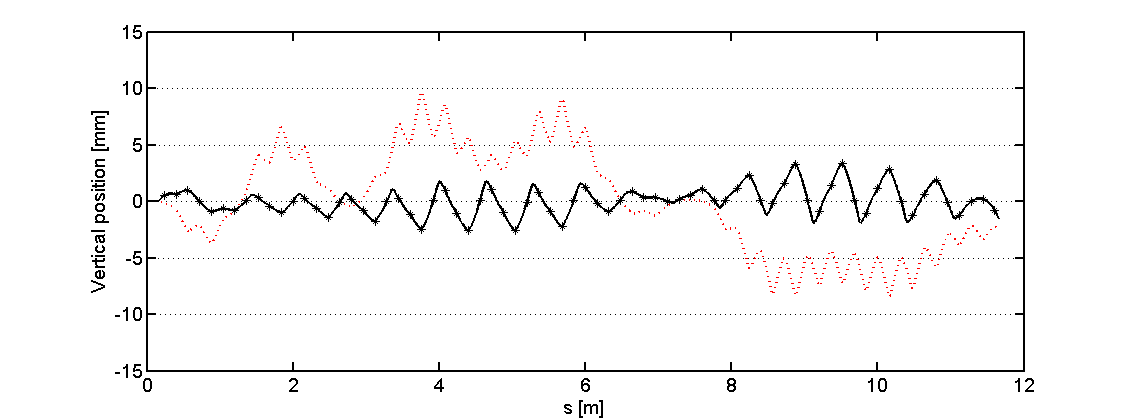
\includegraphics[width=.8\textwidth]{3.figures/steering_rms_y4.png}
     \label{fig:SV_y4}}
\hspace{0.5in}
\subfloat[Vertical steering for perfect alignment, SV current limited to 2 A. ]{
     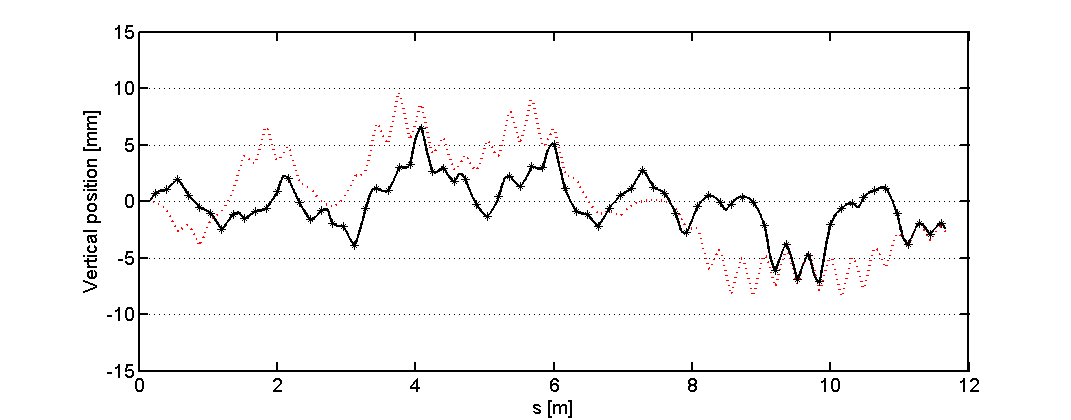
\includegraphics[width=.8\textwidth]{3.figures/steering_rms_y4_CL.png}
     \label{fig:SV_y4_CL}}
\hspace{0.5in}
\subfloat[Vertical steering for misalignment of $\sigma=1$ mm, SV current limited to 2 A.]{
     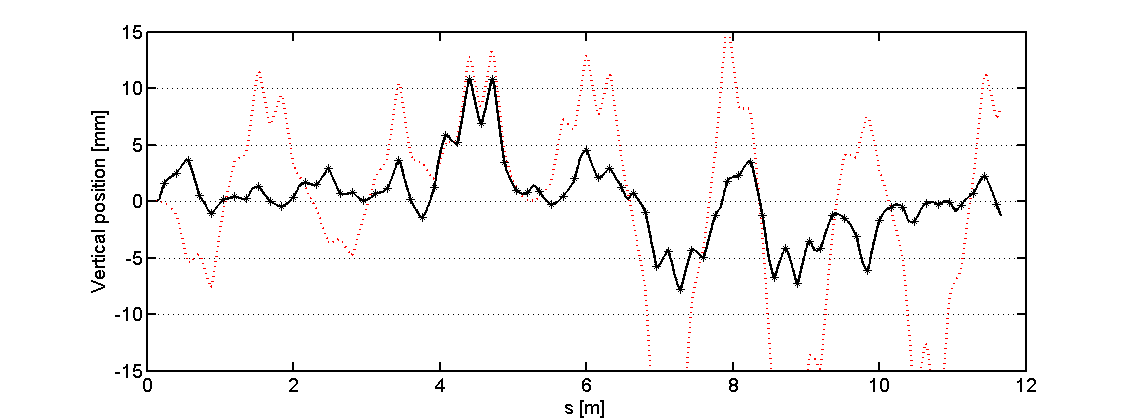
\includegraphics[width=.8\textwidth]{3.figures/steering_rms_y4_misalign1.png}
     \label{fig:SV_y4_misalign}}
\end{figure}




















\section{2D Parameter search for Injection and Recirculation Settings}



\section{Comments on steering the Alternative Lattice}



\section{Implementation}
% This section for technical details of implementation


%% Quad as BPM
The quad as BPM measurement is controlled by UMER control script \newline kiersten\_quad\_scan\_v2.m. 
In this procedure, the current in each ring quadrupole (RQ2-RQ71) is independently scanned about it's nominal 
operating point. The horizontal and vertical position of the nearest downstream BPM is recorded. This data is 
fitted to a linear curve, using the linear least squares method. The fitted slope is the BPM response to the 
quad scan, $\frac{\partial x_{BPM}}{\partial I_{quad}}$, equivalently the uncalibrated position in the quad. 
The errorbars are defined as the 95\% confidence interval of the slope coefficient. 

To calibrate the position in the quad, I use the VRUMER code to determine what initial condition in the quadrupole gives the appropriate BPM response.
I first choose an arbitrary starting position $x_{0,q}$, $x'_{0,q}$ and simulate a quad scan.
I then apply the Newton-Raphson method to determine the appropriate $x_q$ to give the desired (measured) BPM response, $m_{sim} = m_{data}$ (where $m_{data} = \frac{\partial x_{BPM}}{\partial I_{quad}}$): 


\begin{equation}
 x_q = x_{0,q} - \left( m_{sim} - m_{data} \right) \left(\frac{dm_{sim}}{dx_q}\right)^{-1}
\end{equation}

This allows us to define a calibration factor between the BPM response and the position at the center of each quadrupole, 

\begin{equation}
x_q = C_{q,BPM} \times \frac{\partial x_{BPM}}{\partial I_{quad}}
\end{equation}


While this factor will not change for a static version of VRUMER, the \newline  kiersten\_quad\_scan\_v2.m procedure is 
set up to do the Newton-Raphson calculation for every set of quad scan data. This was mainly a matter of convenience at 
the time, as having a lookup table for the calibration factors would result in slight decrease in run time and a loss of 
flexibility (changes to ring operation would require recalculation of the look-up table, etc). Running VRUMER takes $\sim 0.06$ 
seconds, so even for the an entire quad scan (9 points) repeated twice for the Newton-Raphson calculation VRUMER 
costs $\sim 1$ second per quad. 



%% Steering approach
This is a description of the horizontal steering method I used to steer the 6 mA beam on November, 2015. The final solution was saved as settings file kiersten\_6mA\_151116.csv.

The procedure for horizontal steering attempts to steer the beam as close as possible to the center of the quads in the first turn, and use two dipoles at the end of the ring to close the orbit. I generated this solution using an existing solution with many turns, but it should be possible to apply this method to a ring with "no-steering" (significant current loss in the first few turns).
The procedure is as follows:

\begin{enumerate}
\item Set last 2 injection dipoles by scanning currents and identifying smallest rms deviation in first two RQ's after injection. Time: 1 hour.
\item Steer through RQ3 (first turn) by setting current in D1; Repeat injection scan if change was significant. Time: 10 minutes + 1 hour if repeating injection scan.
\item Steer through quads in first turn, setting dipoles D2-34 in order and using quad-as-BPM method to measure position in quads. Time: 2 1/2 hours ($\times 2$ for best results).
\item Close orbit by scanning D34 and D35 currents.  Time: 30 minutes
\item Verify orbit quality by running quad scan for 1st turn quad-as-BPM data, and look at multi-turn BPM data to estimate orbit excursions from closed orbit. Time: 30 minutes.
\end{enumerate}

 Total (minimum) time for steering: $\approx 6$ hours. Time estimates are for total measurement/ beam-on time, more time should be added for trouble-shooting and general unruly behavior.
 
 
 
 
 
 
 
 
 
 
 
 
 %%%%%% closing orbit
\subsection{Closing the orbit}

The final step is to set the current in the dipoles near the end of the ring so that the closed orbit is close to the p1 closed orbit.  Two dipoles are required for control of x and x'. Naively, one would vary the last two dipoles, D35 and PD-Rec. Unfortunately PD-Rec has significant coupling with the first turn beam position. For a scan of PD-Rec from $8.25 \rightarrow 13.75$ A, the position of the beam in the first BPM varies in the range $\Delta x = \pm 2$mm. Changing PD-Rec would mean changing all ring dipole settings to compensate, which is undesirable. 

It is possible but difficult to optimize the value of PD-Rec. Instead, I assume that the present setting (PD-Rec I$=11$ A) is reasonably close to the ideal value such that closing the orbit with D34 and D35 will result in a bump in the closed orbit in that neighborhood. It may be possible to infer, based on the difference in the D34 currents optimized for a) steering through RQ69 and RQ70 and b) a closed orbit solution, the size of the orbit bump. 

To set D34 and D35, I scan the currents in each and record the BPM response for the first four turns in the first 3 BPMs. I try to minimize the RMS change in position between turn 1 and turn $N\le4$ in the first three BPM's. For each BPM 1-3, I define an RMS quantity $\sqrt{\frac{1}{3}\left[ \left(x_2-x_1\right)^2+\left(x_3-x_1\right)^2+\left(x_4-x_1\right)^2\right]}$. In order to find a good closed orbit, I ran 3 scans, increasing the resolution and/or re-centering the scan range for each successive scan. Scan takes $\sim$13 minutes to read 3 BPMs for 11 current settings in each dipole. 

\begin{figure}[htb]
\centering
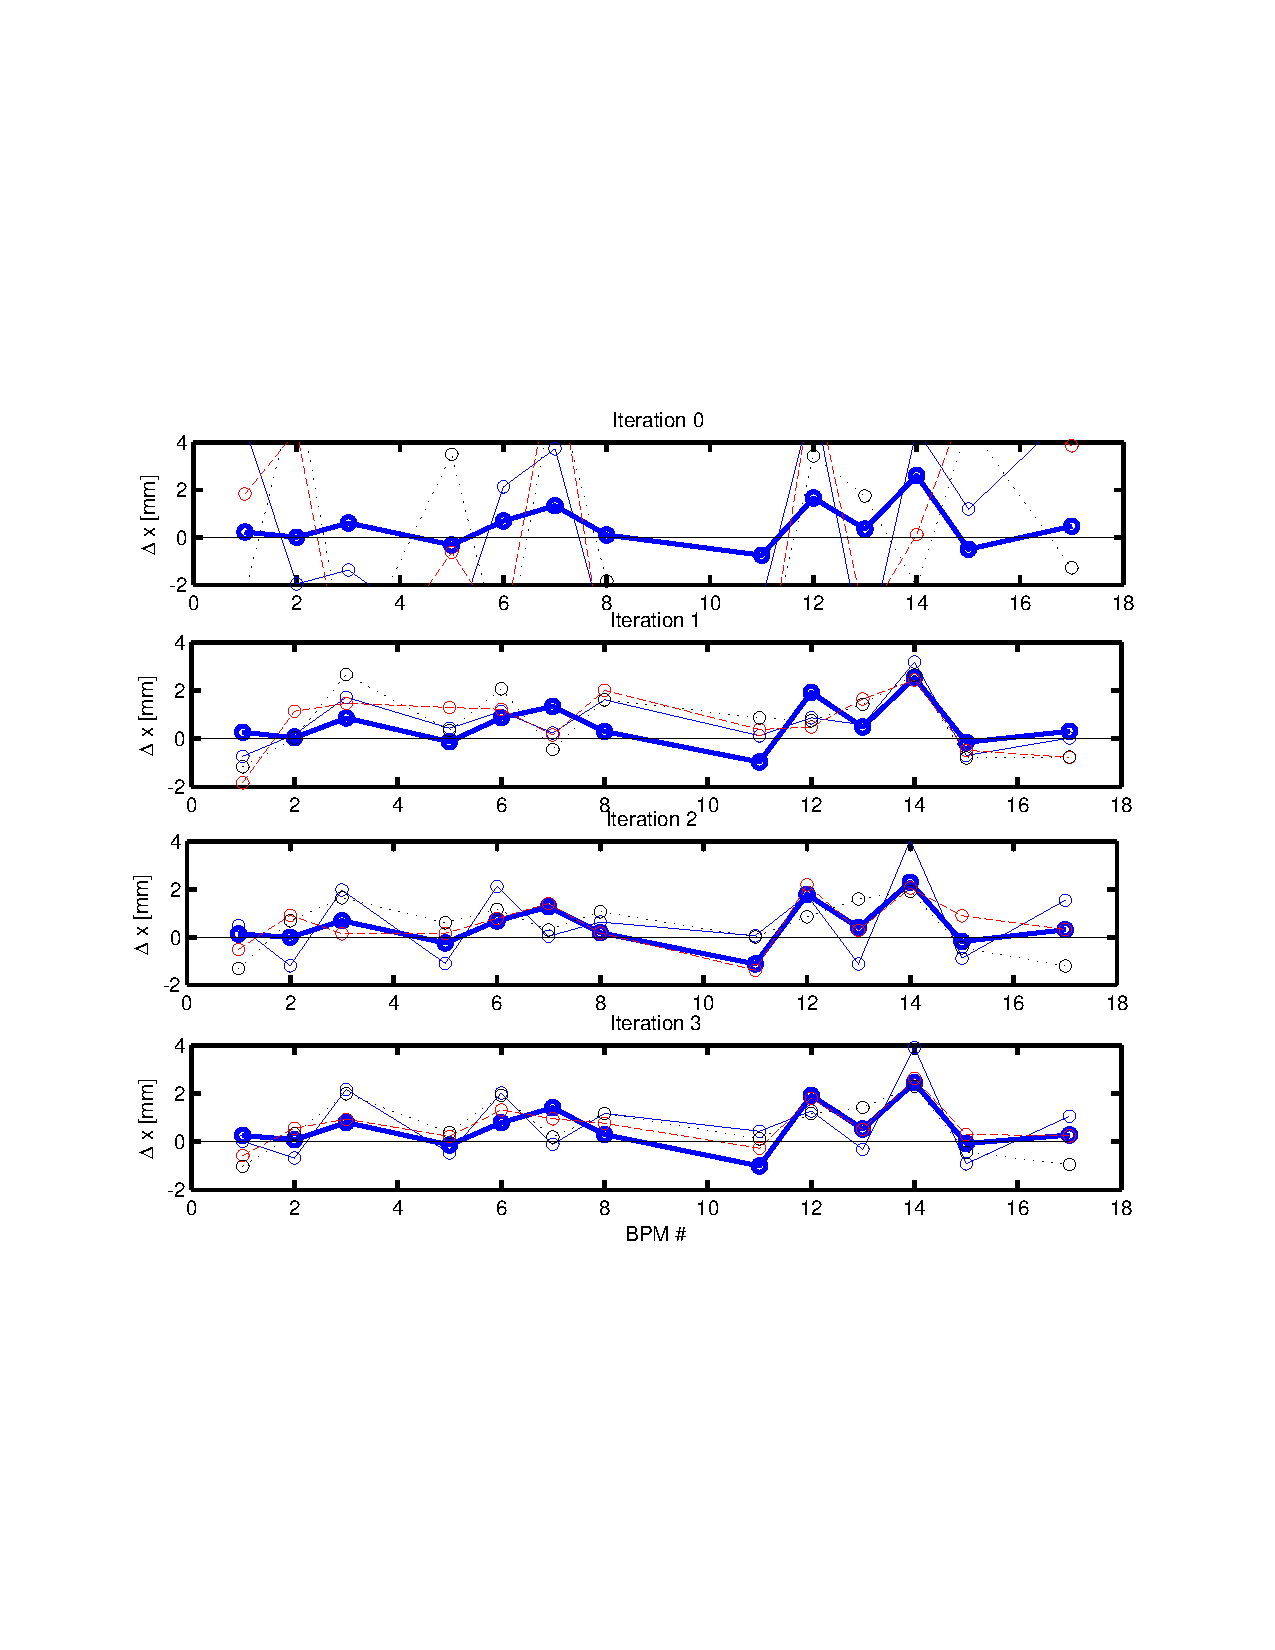
\includegraphics[width=\textwidth,trim={.5in 2.7in .5in 2.7in},clip]{3.figures/closing_orbit_BPMs.pdf}
\caption{BPM response for first 4 turns, for D34, D35 currents listed in table \ref{tab:close_ring}. 1st turn: heavy blue trace. 2nd turn: solid blue. 3rd turn: long dash red. 4th turn: short dash black.}
\label{fig:close_BPMs}
\end{figure}

\begin{figure}[htb]
\centering
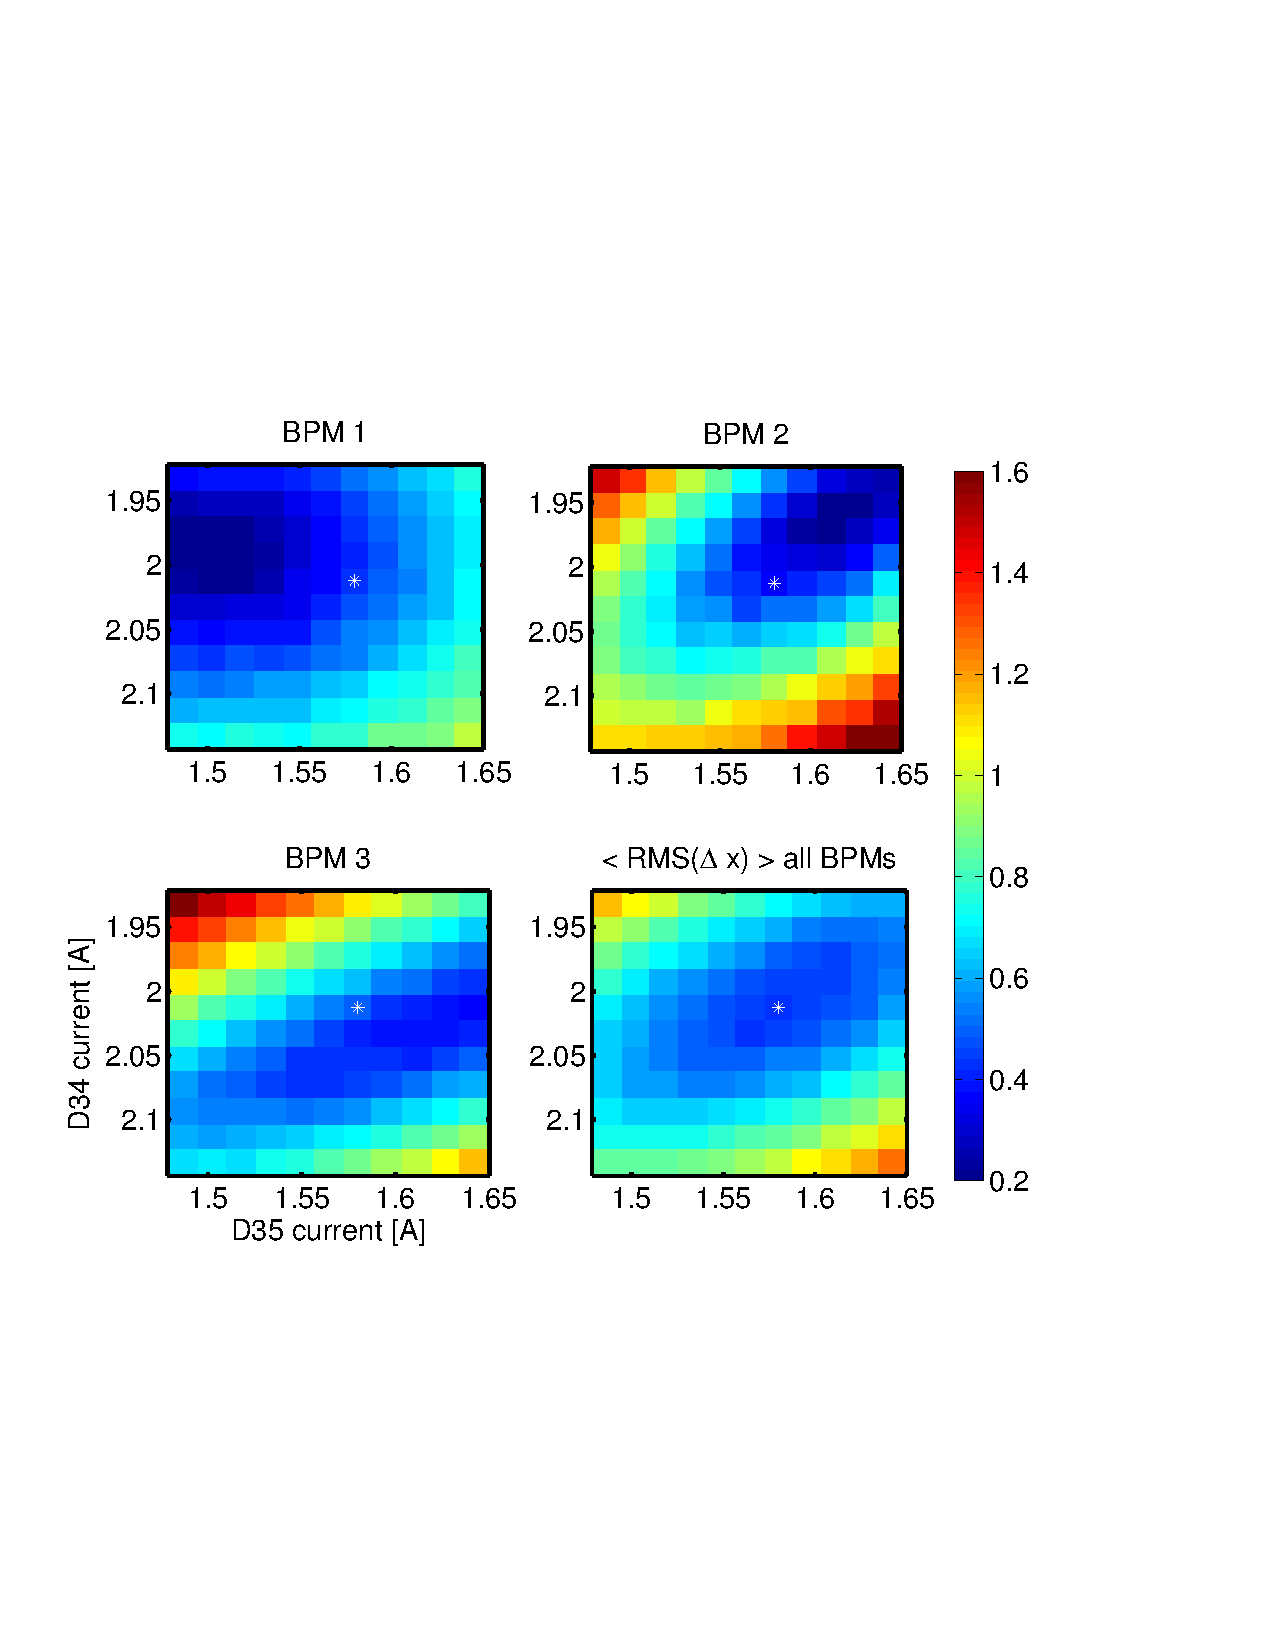
\includegraphics[width=\textwidth,trim={0 2.7in 1in 2.7in},clip]{3.figures/closing_orbit_iteration3.pdf}
\caption{Scan results for first 3 BPMs for iteration 3 in table \ref{tab:close_ring}. Color scale is rms value of $\Delta x$ over first 4 turns [mm], white asterisk indicates optimal setting (D34=2.0129 A, D35=1.5802 A) }
\label{fig:close_scan}
\end{figure}








% Bibliography
\renewcommand{\baselinestretch}{1}
\small\normalsize

\newpage
\bibliographystyle{unsrt} 
\bibliography{thesis} 


\end{document}

